% Created 2024-01-07 Sun 14:28
% Intended LaTeX compiler: xelatex
\documentclass[11pt,twoside,landscape]{article}
\usepackage{graphicx}
\usepackage{longtable}
\usepackage{wrapfig}
\usepackage{rotating}
\usepackage[normalem]{ulem}
\usepackage{amsmath}
\usepackage{amssymb}
\usepackage{capt-of}
\usepackage{hyperref}
\usepackage{subcaption}
\usepackage[newfloat]{minted}
\usepackage{color}
\usepackage{listings}
\usepackage[top=2cm,bottom=2cm,right=2cm,left=2cm,landscape]{geometry}
\usepackage{multicol}
\usepackage{enumitem}
\usepackage{fancyhdr}
\usepackage{caption}
\usepackage{algorithm}
\usepackage{algpseudocode}
\usepackage{float}
\setlist[description]{itemsep=-1pt,leftmargin=2mm,topsep=0pt}
\setlist[itemize]{itemsep=-1pt,topsep=0pt}
\setlist{noitemsep}
\setlength{\parindent}{0pt}
\setlength{\columnseprule}{0.2pt}
\definecolor{mygreen}{rgb}{0,0.6,0}
\definecolor{mygray}{rgb}{0.5,0.5,0.5}
\definecolor{mymauve}{rgb}{0.58,0,0.82}
\lstset{ backgroundcolor=\color{white}, basicstyle=\footnotesize, breaklines=true, captionpos=b, commentstyle=\color{mygreen}, escapeinside={\%*}{*)},keywordstyle=\color{blue}, stringstyle=\color{mymauve},}
\author{Olivier Lischer}
\date{\today}
\title{WE3 Summary}
\hypersetup{
 pdfauthor={Olivier Lischer},
 pdftitle={WE3 Summary},
 pdfkeywords={},
 pdfsubject={},
 pdfcreator={Emacs 29.1 (Org mode 9.7-pre)}, 
 pdflang={English}}
\begin{document}

\pagestyle{fancy}
\fancyhf{}
\fancyhead[R]{FP-FS22}
\fancyhead[L]{Exam Summary}
\fancyfoot[CE,CO]{\leftmark}
\fancyfoot[R]{\thepage}
\fancyfoot[L]{Olivier Lischer}

\begin{multicols}{3}
\section{SPA}
\label{sec:orgfb10ebc}
\subparagraph{What are the benefits of a browser based application?} \
\label{sec:org70e1ce9}
A browser based application (web application) has various benefits:
\begin{itemize}
\item You can work from anywhere at anytime
\item It is platform independent (even mobile)
\item No software update nor installation => easy maintenance
\item Software can provided as a Services (SaaS)
\item Can be cross-compiled to different ecosystems
\begin{itemize}
\item Client app: electron.io
\item Moile app: Native Script / Ionic
\item Server app: "Universal" Compilation
\end{itemize}
\end{itemize}
\subparagraph{What are the liabilities of a browser based application?} \
\label{sec:org682cfbb}
Browser based applications do not have only benefits (\href{../../../roam/20231228101744-what_are_the_benefits_of_a_browser_based_application.org}{What are the benefits of a browser based application?}) but also downsides, such as:
\begin{itemize}
\item no data sovereignty
\item limited / restricted hardware access (no OS access, may be less efficient)
\item Search Engine Optimization (SE must execute JS)
\item More complex deployment strategies
\item Overhead
\end{itemize}
\subparagraph{What is a Single Page Application?} \
\label{sec:org9d193f9}
An SPA is a special kind of \href{../../../roam/20210921092018-web_apps.org}{Web apps}.

\begin{quote}
A Single Page Application (SPA) is a web site [\ldots{}] that fits on a single web page with the goal of providing a user experience
similar to that of a desktop application.
In an SPA, either all necessary code [\ldots{}] is retrieved with a single page load or the
appropriate resources are dynamically loaded and added to the page as necessary.

SPAs use AJAX and HTML5 to create responsive Web apps, without constant page reloads.
-- Wikipedia
\end{quote}
\subparagraph{The traditional web application architecture} \
\label{sec:org7a1eeab}

{
\begin{center}
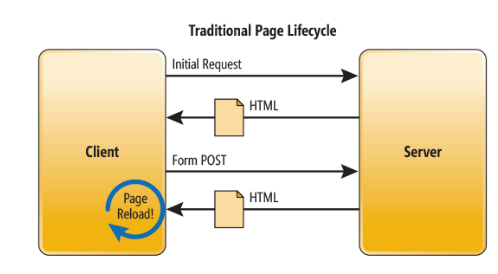
\includegraphics[width=.9\linewidth]{img/traditional_architecture.png}
\end{center}
\captionof{figure}{Traditional Architecture}\label{fig:traditional-architecture}
}
\subparagraph{The SPA architecture} \
\label{sec:org7a5e60a}

{
\begin{center}
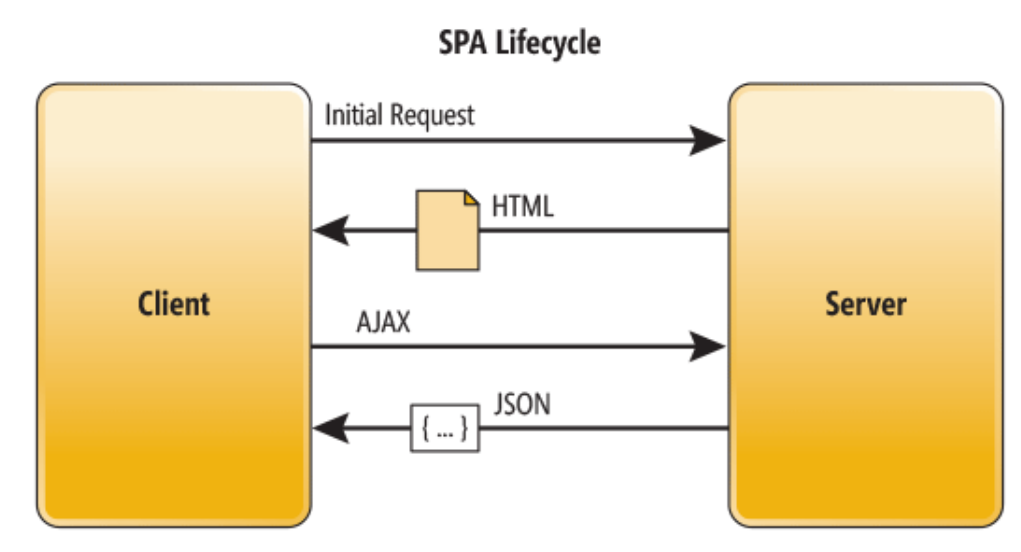
\includegraphics[width=.9\linewidth]{img/spa_architecture.png}
\end{center}
\captionof{figure}{SPA Architecture}\label{fig:spa-architecture}
}
\subparagraph{What are characteristics of an SPA?} \
\label{sec:org8bf7229}
An SPA has the following properties:
\begin{itemize}
\item Plan HTML5 / CSS and JavaScript
\begin{itemize}
\item no plugins like SilverLight or Flash
\end{itemize}
\item no page reloads
\item Working Back-Button
\item Bookmarkable Links
\item Provides (limited) offline functionality
\item Uses (\href{../../../roam/20230108172748-what_is_rest.org}{REST})-API services for data access
\end{itemize}


{
\begin{center}
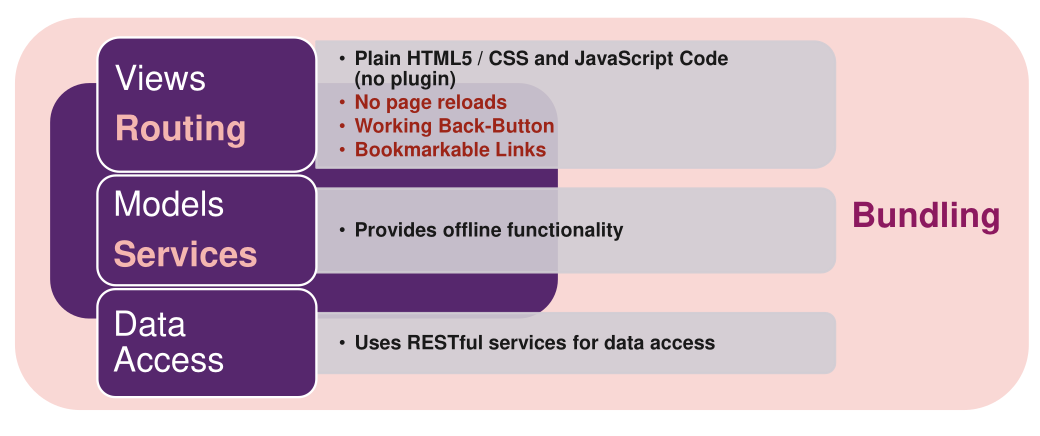
\includegraphics[width=.9\linewidth]{img/spa_logical_overview.png}
\end{center}
\captionof{figure}{Logical Overview of an SPA}\label{fig:logical-overview-of-an-spa}
}
\subparagraph{When would you prefer an SPA to a classic web application from the customer's point of view?} \
\label{sec:orgeb9dba2}
\begin{quote}
As soon as a desktop (native) app with a similar user experience is required.
The page feels like an application.
An SPA also offers more options for complex web applications with lots of animations/graphical elements.
\end{quote}
\subparagraph{What do you see as the technical benefits of an SPA?} \
\label{sec:org84bd33b}

The server application is separated from the display by a structured interface (e.g. REST / ODATA / WSDL). This opens up various advantages:
\begin{itemize}
\item Seperation of Concerns
\item Better maintainability of the client code
\item Division into different teams / competence centers
\end{itemize}
\subparagraph{What does a typical layering in an SPA look like?} \
\label{sec:org478568c}
The Views are connected using a routing in the browser (no new request to the server).
The Business Logic provides data over servies and only the data layer will communicate directly with the server.

{
\begin{center}
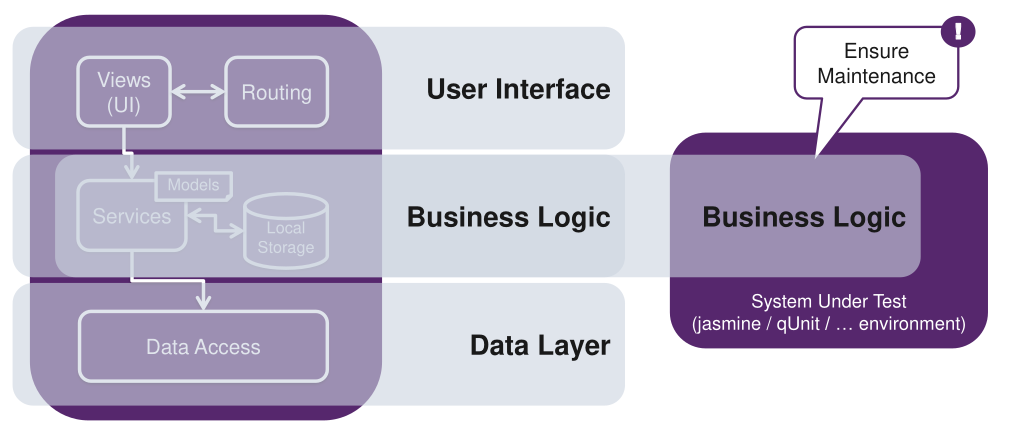
\includegraphics[width=.9\linewidth]{img/spa_layering.png}
\end{center}
\captionof{figure}{Layering in SPA}\label{fig:layering-in-spa}
}
\subparagraph{Why do we use bundling in an SPA?} \
\label{sec:org28ceb9a}
An SPA may consist of many single JS files, which may or may not dependt on each other.
To include them manually in your HTML is error pronce and tedious.

With bundling we achive the following things:
\begin{itemize}
\item All JS code must be delivered to the client over potentially metered/slow networks
\item Bundling and minifying the source leads to smaller SPA footprint (e.g. using \href{../../../roam/20231228113108-what_is_tree_shaking.org}{Tree Shaking})
\item Bundling leads to a reliable dependency management
\item Usage of pre and post processors during bundling
\end{itemize}


The initial footprint caused by bundling can be reduced by loading dependent modules on-demand.
\section{React}
\label{sec:org0689c66}

\subparagraph{What is JSX?} \
\label{sec:orged5272c}
JSX is an extension to JavaScript.
It is used to write markup for an \href{../../../roam/20231228102611-what_is_a_single_page_application.org}{SPA}.
The JSX is transpiled during building into standard ECMAScript

\begin{quote}
JSX is an XML-like syntax extension to ECMAScript without any defined semantics.
It's NOT intended to be implemented by engines or browsers.
It's NOT a proposal to incorporate JSX into the ECMAScript spec itself.
It's intended to be used by various preprocessors (transpilers) to transform these tokens into standard ECMAScript. 
-- facebook.github.io/jsx/
\end{quote}
\subparagraph{How is JSX desugared in React?} \
\label{sec:orgb08c657}
\begin{listing}[htbp]
\begin{minted}[]{js}
import React from 'react'

function Container(props) {
  return
  className="container">
    {props.children}
  </div>
}
\end{minted}
\caption{\label{lst:jsx}JSX}
\end{listing}

\begin{listing}[htbp]
\begin{minted}[]{js}
function Container(props) {
  return React.createElement(
    "div",
    {className:"container"},
    props.children
  )
}
\end{minted}
\caption{\label{lst:desugared-jsx}Desugared JSX}
\end{listing}
\subparagraph{How do you make props available for all child components?} \
\label{sec:org9f7d811}
Some props must be availabel in all components (e.g. color scheme).
It does not scale well, if you have to pass all props from the root component.
To solve this problem, we can use contexts.
However, you should only use contexts for read-only variables and limit the number of different contexts.



\begin{minted}[]{js}
const themes = {
  light: {
    foreground: "#000000",
    background: "#eeeeee",
  },
  dark: {
    foreground: "#ffffff",
    background: "#222222",
  },
};
const ThemeContext = React.createContext(themes.light);

function App() {
  return (
    <ThemeContext.Provider value={themes.dark}>
      <Toolbar />
    </ThemeContext.Provider>
  );
}

function ThemedButton() {
  const theme = useContext(ThemeContext);
  return (
    <button style={{
              background: theme.background,
              color: theme.foreground }}>
      {" "}I am styled by theme context!{" "}
    </button>
  );
}
\end{minted}
\subparagraph{How does Redux work?} \
\label{sec:orgdfbc521}
The state in Redux is represented as trees of objects.
The tree is immutable.
When you change something in the tree, a new tree will be created (\href{../../../roam/20220616080932-functional_programming.org}{Functional Programming}).

A state action is communicated using a \emph{Redux Action}.
A \emph{Reducer} takes the action and the current state an applies the action on the state to generate a new state.

\begin{figure}[htbp]
\centering
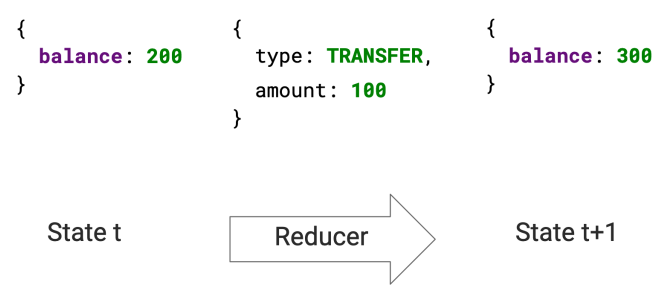
\includegraphics[width=.9\linewidth]{img/redux_action_reducer.png}
\caption{\label{fig:action-reducer-state-change}Action Reducer State change}
\end{figure}
\section{Angular}
\label{sec:orgc174dc9}
\section{ASP.NET}
\label{sec:org54f4898}


\end{multicols}
\end{document}
